\documentclass[12pt,fleqn]{article}\usepackage{../../common}
\begin{document}
Sezonsallık, Trend Çıkartmak, Değişim Noktası


\begin{minted}[fontsize=\footnotesize]{python}
import pandas as pd
series = pd.read_csv('daily-min-temperatures.csv', header=0,\
                      index_col=0, parse_dates=True)
X = [i%365 for i in range(0, len(series))]
y = series.values
degree = 4
coef = np.polyfit(X, y, degree)
curve = [np.sum([coef[-1]] + [x**(degree-d)*c for d,c \
         in enumerate(coef[:-1])]) for x in X]
series['curve']  = curve
series.plot()
plt.savefig('tser_022_de_01.png')
\end{minted}






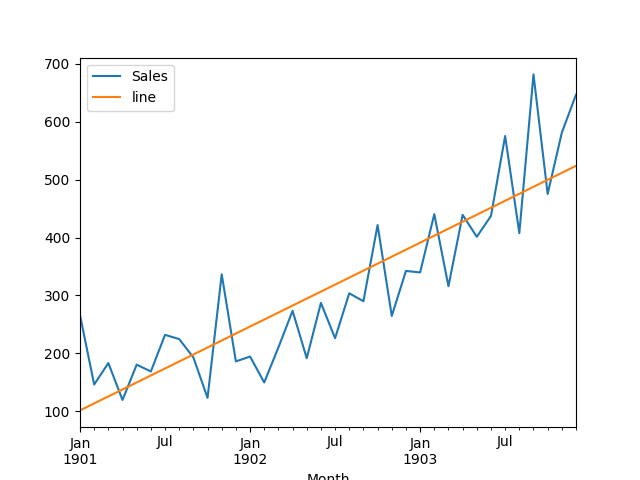
\includegraphics[height=6cm]{tser_022_de_01.png}




 















\end{document}
